\chapter{Improving SMT Model}
\section{Gathering More Data} % PROVIDE 5 CITATIONS TOTAL
The first thing I did to improve the SMT model described in this paper is to gather more high-quality Kinyarwanda | English translation data ad formatting it in the right way so that I could add to data from the Bible that I already had. To do this, I started by gathering translated texts from various on-line sources such as news articles, blog posts, encyclopedia entries, etc. But this wasn't enough as most of these translations either contained some mistakes that I had to manually correct or they were not ready for direct use as they were incorrectly formatted and I had to copy paste them into files, and check line by line to make sure they are well-formatted; and this was quite a lot of work for one person, and there was no going around it because from what I understand, having incorrect data would corrupt the translation model and this would easily lead to several erroneous and inaccurate translation results. 
\section{Kinyarwanda Online}
Having realized that I couldn't possibly complete the process of gathering data on my own, I went ahead and set up a translations crowd-sourcing website. On the website provided, I provided a list of the most used English sentences, I asked Kinyarwanda and English bilingual users to provide translations to as many sentences as they can. This initiative did not go well as I planned as only few people participated. The website is still on-line at this link:  \url{http://kinyarwanda.online/}, and I am still waiting for more translations to added by users with the hope that one day I or someone else can use the data gathered from the website to develop a new Kinyarwanda | English translation system and/or help improve existing ones such as \textit{Google Translate}\footnote{Kinyarwanda is one of the languages under development by Google Translate. Volunteers can contribute by providing or validating translations at \url{https://translate.google.com/about/intl/en_ALL/contribute.html}} and \textit{SmartRwanda}\footnote{\url{https://smartrwanda.org/translate}}.

\begin{figure}[h]
\begin{center}
\captionsetup{justification=centering}
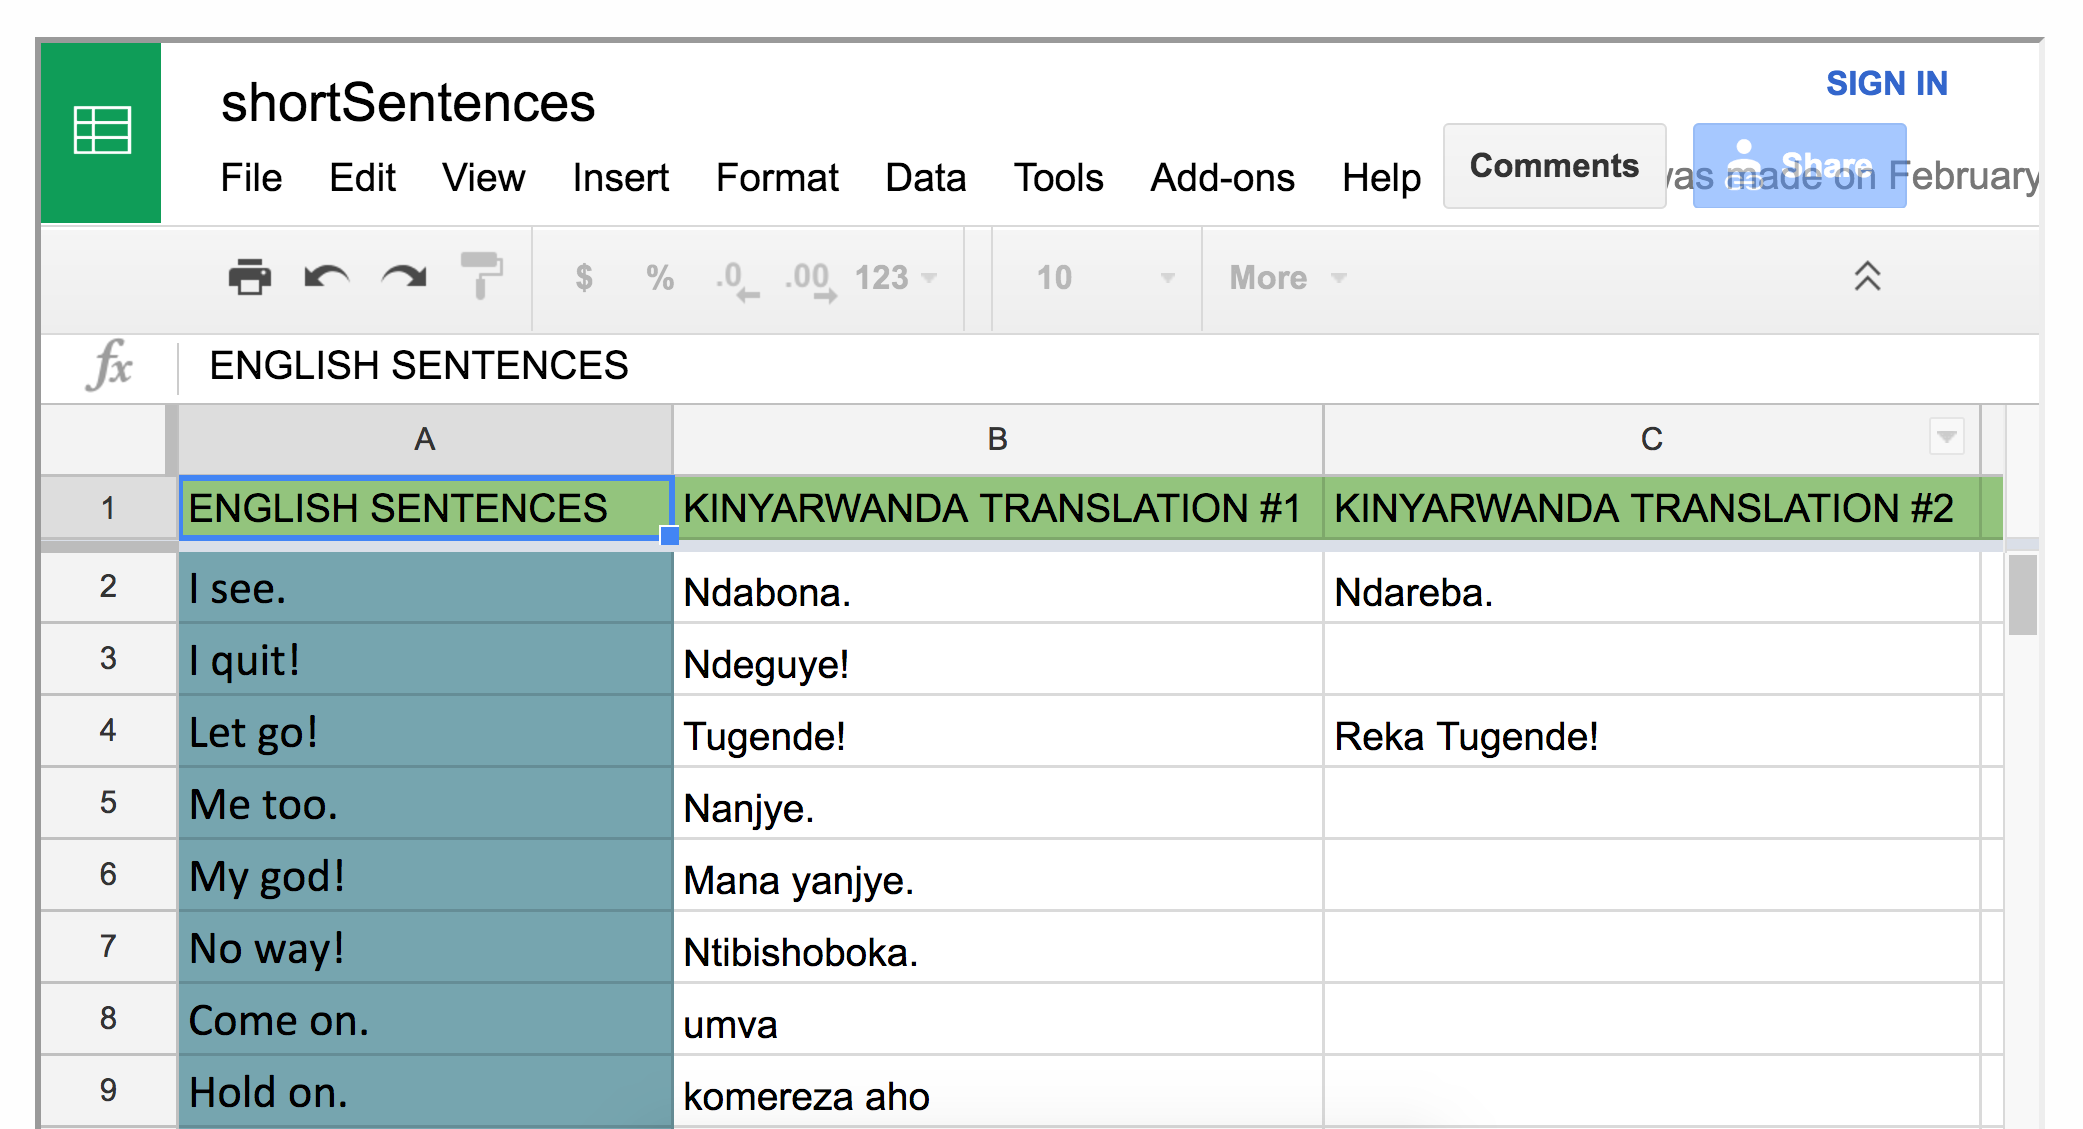
\includegraphics[width=6in]{figures/kinyarwanda-online-spreadsheet.png}
\caption{A preview of the spreadsheet containing crowd-sourced translation data. 
Image Source: \protect\url{http://kinyarwanda.online/translate/}. Screenshot taken on March 29, 2017.}
\end{center}
\end{figure}